%%%%%%%%%%%%%%%%%%%%%%%%%%%%%%%%%%%%%%%%%%%%%%%%%%%%%%%%%%%
%% Congratulations, you've made an excellent choice
%% of writing your Tampere University thesis using
%% the LaTeX system. This document attempts to be
%% as complete a template as possible to let you focus
%% on the most important part: the writing itself.
%% Thus the details regarding the visual appearance
%% and even structure have already been worked out
%% for you!
%%
%% I sincerely hope you will find this template useful
%% in completing your thesis project. I've tried to
%% add comments (followed by the % sign) to clarify
%% the structure and purpose of some of the commands.
%% Most of the magic happens in the file tauthesis.cls,
%% which you are more than welcome to take a look at.
%% Just refrain from editing it in the most crucial
%% versions of the thesis!
%%
%% I wish you and your thesis project the best of luck!
%% If this template causes you trouble along the way
%% or if you've any suggestions for improving it,
%% please be in contact through GitHub
%% (<URL HERE>)
%%
%% Yours,
%%
%% Ville Koljonen
%%
%% PS. This template or its associated class file don't
%% come with a warranty. The content is provided as is,
%% without even the implied promise of fitness to the
%% mentioned purpose. You, as the author of the thesis,
%% are responsible for the entire work, including the
%% provided material. No one else is liable to you for
%% any damage inflicted on you or your thesis, were it
%% caused by using this template or not.
%%%%%%%%%%%%%%%%%%%%%%%%%%%%%%%%%%%%%%%%%%%%%%%%%%%%%%%%%%%

%%%%% NOTICE %%%%%
%% Please read through the entire template
%% (files under ./tex) to find all instructions.
%% It is possible that the attached pdf files
%% do not include the latest information.
%%%%%%%%%%%%%%%%%%

%%%%% INSTRUCTIONS FOR COMPILING THE DOCUMENT %%%%%
%% Overleaf: just click Recompile.
%% Terminal:
%%  1. pdflatex main.tex
%%  2. makeindex -s main.ist -t main.glg -o main.gls main.glo
%%  3. biber main
%%  4. pdflatex main.tex
%%  5. pdflatex main.tex
%% Similar sequence of commands is also required
%% in LaTeX specific editors.
%%%%%%%%%%%%%%%%%%%%%%%%%%%%%%%%%%%%%%%%%%%%%%%%%%%

%%%%% METADATA %%%%%
%% Always keep the following metadata up to date!
%% This is important for your PDF file to comply
%% to accessibility standards.
%% (And yes, this information must remain here,
%% before \documentclass[...]{...}.)

% \Title and \Language are mandatory,
% others desirable
% The appropriate Finnish language code is 'fi',
% UK English is en-UK
\begin{filecontents*}[overwrite]{\jobname.xmpdata}
\Title{HapSynth}
\Author{Ville Helppolainen}
\Language{en-US}
\end{filecontents*}

\pdfminorversion=6

%%%%% PREAMBLE %%%%%

%%%%% Document class declaration.
% The possible optional arguments are
%   finnish - thesis in Finnish (default)
%   english - thesis in English
%   numeric - citations in numeric style (default)
%   authoryear - citations in author-year style
%   apa - citations in APA 7 (available only in English)
%   ieee - citations in IEEE style (available only in English)
%   draft - for faster non-final works, also skips images
%           (recommended, remove in final version)
%   programs - if you wish to display code snippets
% Example: \documentclass[english, authoryear]{tauthesis}
%          thesis in English with author-year citations
\documentclass[english, apa]{tauthesis}

% The glossaries package throws a warning:
% No language module detected for 'finnish'.
% You can safely ignore this. All other
% warnings should be taken care of!

%%%%% Your packages.
% Before adding packages, see if they can be found
% in tauthesis.cls already. If you're not sure that
% you need a certain package, don't include it in
% the document! This can dramatically reduce
% compilation time.

% Graphs
% \usepackage{pgfplots}
% \pgfplotsset{compat=1.15}

% Subfigures and wrapping text
% \usepackage{subcaption}

% Mathematics packages
\usepackage{amsmath, amssymb, amsthm}
%\usepackage{bm}

% Chemistry packages
% \usepackage{chemfig}
% \usepackage[version=4]{mhchem}

% Text hyperlinking
% \usepackage{hyperref}
% \hypersetup{hidelinks}

% (SI) unit handling
% \usepackage{siunitx}

\usepackage{tabularx}
\renewcommand\tabularxcolumn[1]{m{#1}}
\newcommand*{\thead}[1]{\bfseries\hspace*{\fill}{#1}\hspace*{\fill}}

\usepackage{multirow}

\usepackage{svg}
\usepackage{csvsimple}

\usepackage{pdflscape}

\usepackage{placeins}

\usepackage{todonotes}
\newcommand\todox[1]{\todo[size=\tiny]{#1}}

%\sisetup{
%    detect-all,
%    math-sf=\mathrm,
%    exponent-product=\cdot,
%    output-decimal-marker={,} % for theses in FINNISH!
%}

%%%%% Your commands.

% Print verbatim LaTeX commands
\newcommand{\verbcommand}[1]{\texttt{\textbackslash #1}}

\DeclareUnicodeCharacter{03C3}{$\boldsymbol{\sigma}$}

% Basic theorems in Finnish and in English.
% Remove [chapter] if you wish a simply
% running enumeration.
% \newtheorem{lause}{Lause}[chapter]
% \newtheorem{theorem}[lause]{Theorem}

% \newtheorem{apulause}[lause]{Apulause}
% \newtheorem{lemma}[lause]{Lemma}

% Use these versions for individually
% enumerated lemmas
% \newtheorem{apulause}{Apulause}[chapter]
% \newtheorem{lemma}{Lemma}[chapter]

% Definition style
% \theoremstyle{definition}
% \newtheorem{maaritelma}{Määritelmä}[chapter]
% \newtheorem{definition}[maaritelma]{Definition}
% examples in this style

%%%%% Glossary information.

% Use the following lines ONLY if you need more
% than one glossary. The first argument specifies
% a type label for the glossary and the second
% the displayed name.
% \newglossary*{symbs}{Symbols}
% \newglossary{label}{Displayed name}
% ...

\makeglossaries

% Use this line if using the default glossary.
% Otherwise comment out.
\loadglsentries[main]{tex/glossary.tex}

% Use this line if using more than one glossary.
% Otherwise comment out.
% \loadglsentries[symbs]{tex/sanasto2.tex}

%%%%% Citation information.

% Commonly used bibliography modifications.
% Feel free to play around with them.

%\ExecuteBibliographyOptions{%
%sorting=none,
%maxbibnames=99,
%maxcitenames=2,
%giveninits=true,
%uniquename=init,
%sortcites,
%sortlocale=fin}

%\DefineBibliographyStrings{finnish}{%
%    in = {},
%    pages = {s.},
%    page = {s.}
%}
%\DefineBibliographyStrings{english}{%
%    in = {},
%    pages = {pp.},
%    page = {p.}
%}
%
%\DeclareNameAlias{sortname}{last-first}
%\DeclareNameAlias{author}{last-first}

%\DeclareFieldFormat[%
%    article,inbook,incollection,inproceedings,
%    patent,thesis,unpublished]{citetitle}{#1\isdot}
%\DeclareFieldFormat[%
%    article,inbook,incollection,inproceedings,
%    patent,thesis,unpublished]{title}{#1\isdot}
%\DeclareFieldFormat{pagetotal}{#1 \bibstring{page}}

%\AtBeginBibliography{\renewcommand*{\makelabel}[1]{#1\hss}}

%\DefineBibliographyExtras{english}{\let\finalandcomma=\empty}

\addbibresource{tex/references.bib}

\begin{document}

%%%%% FRONT MATTER %%%%%

\frontmatter

%%%%% Thesis information and title page.

% The titles of the work. If there is no subtitle,
% leave the arguments empty. Pass the title in
% the primary language as the first argument
% and its translation to the secondary language
% as the second.
\title{HapSynth}{}
\subtitle{Utilizing force feedback on digital musical instruments}{}

% The author name.
\author{Ville Helppolainen}

% The examiner information.
% If your work has multiple examiners, replace with
% \examiner[<label>]{<name> \\ <name>}
% where <label> is an appropriate (plural) label,
% e.g. Examiners or Tarkastajat, and <name>s are
% replaced by the examiner names, each on their
% separate line.
\examiner[Examiners]{Ahmed Farooq \\ Jari Kangas}

% The finishing date of the thesis (YYYY-MM-DD).
\finishdate{2024}{05}{21}

% The type of the thesis (e.g. Kandidaatintyö
% or Master of Science Thesis) in the primary
% and the secondary languages of the thesis.
\thesistype{Master of Science Thesis}{}

% The faculty and degree programme names in
% the primary and the secondary languages of
% the thesis.
\facultyname{Faculty of Information Technology and Communication Sciences}{}
\programmename{Master's Degree Programme in Human-Technology Interaction}{}

% The keywords to the thesis in the primary and
% the secondary languages of the thesis
\keywords%
    {haptics, force feedback, digital musical instruments}
    {}

\maketitle

%%%%% Abstracts and preface.

% Write the abstract(s) and the preface
% into a separate file for the sake of clarity.
% Pass the appropriate file name as the first
% argument to these commands. Put the \abstract
% in the primary language first and the
% \otherabstract in the secondary language second.
% Those who do not speak Finnish only need the
% first abstract. The second argument of
% the \preface command takes the place where
% the thesis was signed in.
\abstract{tex/abstract.tex}
% \preface{tex/preface.tex}{At Tampere}

%%%%% Table of contents.

\tableofcontents

%%%%% Lists of figures, tables, listings and terms.

% Print the lists of figures and/or tables.
% Uncomment either of these commands as required.
% Both are optional, but if there are many important
% figures/tables, listing them may be a good idea.

% \listoffigures
% \listoftables
% \lstlistoflistings

% Misc stuff related to how the glossary is displayed.
% You can especially tweak the lengths to suit you!
\glsaddall
\setglossarystyle{taulong}
\setlength{\glsnamewidth}{0.25\textwidth}
\setlength{\glsdescwidth}{0.75\textwidth}
\renewcommand*{\glsgroupskip}{}

% Print the default glossary of abbreviations,
% if necessary. Otherwise comment out.
% The appropriate Finnish variant is 'Lyhenteet'
\printglossary[title={Glossary}]

% Print more than one glossary with these lines.
% Otherwise comment out.
% \printglossary[type=symbs]
% \printglossary[type=label]
% ...

%%%%% MAIN MATTER %%%%%

\mainmatter

\chapter{Introduction}
\label{ch:introduction}
\glspl{dmi}, or synthesizers in layman terms, are great instruments for making a variety of different sounds. Unlike traditional instruments that produce sound by directly vibrating the air with i.e. a string or a membrane, they generate electrical signals that represent the audio waves. This causes \glspl{dmi} to inherently lose to traditional instruments in tactility, and all forms of primary feedback must be intentionally designed.

With older \glspl{dmi} each parameter of the \gls{synth} was exposed as a dedicated input in the user interface, i.e. as a button, knob, or slider, and thus had a "knob-per-function" interface. This allowed each input, and as a by-product each parameter, to have unique feel, or tactile feedback. Depending on what the designer of the instrument wanted, some knobs could turn smoothly while others could have more resistance, some sliders could stay on the position they were set in while others could spring back to the initial position, and most prominently some inputs could move freely while others could have discreet steps or detents they lock in. This helps the player to control the instruments more efficiently, as they can trust their fingers in addition to their eyes and ears.

However, modern, especially digital, synthesizers contain more and more functions, and it is physically impossible to fit a dedicated input for each parameter while still having a reasonably sized instrument. Thus, inevitably some inputs must alternate in controlling multiple parameters, which causes the feel of the inputs to become generic. Players can't depend on their fingers anymore, instead they need to look for visual indicators, usually led lights or small displays, to see what they are changing and how much.

Meanwhile various motorized inputs were surfacing to consumer markets in the start of 2020s. Notably Sony PlayStation 5's DualSense controller introduced adaptive triggers with force feedback for a wide audience, being able to change the resistance of the triggers depending on situation and simulate interaction with physical objects like pushing car's brake pedal or shooting a bow. Also music gear segment saw the same introduction of motorized inputs. subMatrix's Beettweek (\cite{submatrix2024}) and Der Mann mit der Maschine's M4 (\cite{dmm2024}) were two new interesting \gls{dmi} controllers having motorized knob and sliders respectively, providing various force feedback modes. Furthermore, Melbourne Instruments announced Nina (\cite{melbourneinstruments2024}), a fully featured synthesizer with over 30 motorized knobs, representing the current cutting edge of force feedback enabled synthesizers.

Motorized inputs can't solve the problem of one input controlling multiple parameters, but they might be beneficial by allowing the feel of the input change depending on the edited parameter. In this study I aim to find out whether that is the case or not. On the basis of past research, I will create an open source (see Appendix \ref{ch:links}) \gls{dmi} with force feedback enabling motorized slider, which I then use to conduct a user research. By combining qualitative and quantitative research methods I examine if force feedback has an effect to a user's subjective experience of usability and enjoyability, and objective measurable performance.

\chapter{Past research}
\label{ch:theory}
\section{Motorized physical sliders and their force feedback modes}

A motorized physical slider is a one-dimensional linear potentiometer, a slider, coupled with a motor. These sliders are usually manufactured to be used i.e. on mixing consoles (\cite{bourns2020}) where the motor is used just to automatically position the slider to a predefined position. However, past research has demonstrated how they can also be utilized to provide users with force feedback by making the motor try to move the slider while the user is moving it, thus applying pressure to the user's fingers (\cite{bak2015, beamish2004, berdahl-kontogeorgakopoulos2013, gillespie-rosenberg1995, papetti2018,kontogeorgakopoulos2019}). By varying the strength and direction of the motor, different force feedback modes can be created.

Student paper \textcite{kretz2004} introduces six force feedback modes for motorized sliders: \textit{Position}, \textit{Elasticity}, \textit{Friction}, \textit{Gradual}, \textit{Texture}, and \textit{Oscillation}. Aside from \textit{Friction}, these modes are rehashed in several later publications, where they are considered basic building blocks which can be combined to create new modes (\cite{jenaro2007, kretz2005, shahrokni2006}). Even though \textit{Friction} mode is missing from those publications, I have decided to include it in this study for completeness. The behaviour of each of these modes are explained in Table \ref{fjeldmodes}. \textit{Gradual} mode is also referred as \textit{Detents}, which is the term I will be using in this thesis.

\begin{table}[h!]
	\centering
	\begin{tabularx}{\textwidth}{ |c|X| }
		\hline
		\thead{Mode} & \thead{Description} \\
		\hline
		Position & Motor is turned off: the slider moves freely, and no force feedback is applied. \\
		\hline
		Elasticity & The slider emulates a rubber band: the more it is displaced from the initial position, the more it "fights back". When released the slider returns to the initial position. \\
		\hline
		Friction & The slider emulates high friction: while initiating a movement the motor applies high counter force, when released the slider stays in place. \\
		\hline
		Detents/Gradual & The slider emulates detents: while moving the slider snaps to discreet positions or "detents". \\
		\hline
		Texture & The slider emulates a rough surface: while moving the motor applies low-intensity vibration to it, thus giving an appearance of a rough surface. \\
		\hline
		Oscillation & The slider emulates damped sine movement: when released it returns to initial position following a damped sine curve. \\
		\hline
	\end{tabularx}
	\caption{Basic force feedback modes for a motorized slider (\cite{kretz2004, jenaro2007}).}
	\label{fjeldmodes}
\end{table}

\section{Electrophones and Digital Musical Instruments}

Electrophones are musical instruments that produce sound by generating an electrical signal that drives a loudspeaker (\cite{mimo2011}). They were first categorized in \textit{A Textbook of European Musical Instruments: Their Origin, History and Character} (\cite{galpin1937}) as \textit{“electrophonic instruments”} and later normalized as \textit{"electrophones"}, the fifth category of Hornbostel-Sachs classification of musical instruments (\cite{lee2019}). While electrophones include instruments such as electric guitars, where acoustic signal is amplified with electric circuitry, and pipe organs, where acoustic signal is heard when electrically controlled valve is opened, in this study I focus on electrophones that generate sound using electrical circuitry only. These instruments overlap with the definition of \glspl{dmi}.

Modern \gls{dmi} research builds on top of \citeauthor{miranda-wanderley2006}'s (\citeyear{miranda-wanderley2006}) \textit{New digital musical instruments: control and interaction beyond the keyboard}\footnote{As of writing, \textit{New digital musical instruments: control and interaction beyond the keyboard} is cited 748 times in total and 124 times in 2020 or later (Google Scholar, fetched 3.4.2023).}, which classifies \glspl{dmi} as instruments which consist of two distinct modules: a \gls{controller} and a \gls{synth}. A user interacts with the \gls{controller} (for example by pushing a button or moving a slider on it), which transforms the interaction to an electrical signal. These signals are mapped to one or more parameters of a \gls{synth}, which uses that information and its own algorithm to generate a sound wave. (\cite{miranda-wanderley2006}.)

\glspl{dmi} provide user with two types of feedback: primary feedback (visual, auditory, and tactile-kinesthetic) from the \gls{controller} and secondary feedback (auditory) from the \gls{synth}. The auditory feedback of the \gls{controller} means the mechanical noises that come from operating the \gls{controller} (such as button clicks), while the feedback from the \gls{synth} is the actual sound wave it generates, making them fundamentally different. With traditional instruments the auditory feedback is often accompanied with tactile feedback, as the user can feel the elements generating the sound (i.e., a string or a membrane) vibrating. This tactile feedback is inherently missing from \glspl{dmi} due to decoupling of \gls{controller} and \gls{synth}. Figure \ref{dmi} visualizes the flow within \gls{dmi} from user interaction to received feedback. (\cite{miranda-wanderley2006}.)

\begin{figure}[h]
	\centering
	\includegraphics[width=0.8\linewidth]{figures/dmi.png}
	\caption{Representation of a \gls{dmi} adapted from \textcite{miranda-wanderley2006}.}
	\label{dmi}
\end{figure}

\textit{Sound synthesis and sampling} (\cite{russ2009}) describes a vast number of sound synthesis techniques used in \gls{synth} part of \glspl{dmi}. \textcite{russ2009} categorizes sound synthesis techniques into five main categorizes: physical, analogue, hybrid, digital, and computer software. Analogue synthesis uses electrical circuitry to generate a continuous electrical signal for representing a sound wave, while digital synthesis uses components like microprocessors to process binary data to represent that. (\cite{russ2009}.) Note that also instruments using analogue synthesis are considered \acrlongpl{dmi}.

Particularly prevalent analogue synthesis technique is "subtractive synthesis", in which sound generation starts with harmonically rich waveform which is then modified with a filter that takes out some of the harmonies, while "analogue modeling" is a digital synthesis technique that emulates subtractive synthesis with digital circuitry (\cite{russ2009}). Modern analogue modeling synthesizers sound very close to their analogue counterparts while often offering more features and/or lower price, which have made them popular among consumers (\cite{russ2009}). In this research I focus on analogue modeling synthesis.

\section{Force feedback with \glspl{dmi}}

Force feedback in the context of \glspl{dmi} has been a subject of research at least from the late 1970s with the pioneering work of \textcite{cadoz1984} demonstrating utilizing motorized slider and piano key to give force feedback to musical gestures performed with them. Over 40 years later the topic still interests researchers as they develop new ways to incorporate force feedback into \glspl{dmi}. For example, \textcite{timmermans2020} continue the work on force feedback enabled piano keys, using a linear actuator coupled with a key to accurately replicate the force feedback action of a grand piano key, while \textcite{kirkegaard2020} introduces an open source platform for designing rotary force feedback \glspl{dmi}.

"FireFader" is another open source platform for designing force feedback \glspl{dmi} utilizing two motorized sliders (\cite{berdahl-kontogeorgakopoulos2013}). In the original research it was demonstrated to emulate a virtual mass hanging from the slider with a spring and plucking of a virtual string (\cite{berdahl-kontogeorgakopoulos2013}), while later studies have found numerous other force feedback utilizing applications for it. \textcite{papetti2018} used multiple FireFaders to form an orchestra, where each FireFader acted as a string instrument one slider being used to pluck virtual strings while other controlled the pitch or timbre of the sound. Likewise, \textcite{kontogeorgakopoulos2019} used multiple FireFaders collaboratively, connecting the sliders with virtual springs allowing performers to feel the slider movement of other performers.

\textcite{beamish2004} demonstrated "Q-Slider", a motorized slider which indicates the position of a song by automatically moving the slider accordingly and allows the user to set the position by moving the slider by hand. While moving the slider, a counter force is applied proportional to the song's amplitude on the slider's position, hence making moving the slider easier on quieter parts of a song and harder on louder parts. This was demonstrated to be a highly effective way to find different parts of a song by feeling. (\cite{beamish2004}.) \textcite{bak2015} display results of classes and workshops about sound synthesis and haptics held from 2011 to 2015. One such result was "Duojam", where two motorized sliders virtually attract each other (\cite{bak2015}).

\chapter{Methodology}
\label{ch:methodology}
\section{Purpose and objectives of the study} \label{purpose}

In this thesis I set out to research the usability of force feedback in the context of \glspl{dmi}. I wanted to find out how the user experience differs in \glspl{dmi} with and without force feedback, especially whether users would find inclusion of force feedback helpful and enjoyable. Sometimes using something new can feel difficult or unpleasant, while in reality it is actually helping the user to reach their goal. That is why in comparison to the subjective experience of the users, I also wanted to see if force feedback could provide any objective, measurable benefit. My research questions are:

\begin{enumerate}
	\item How do users find the helpfulness and enjoyability of using a \gls{dmi} with force feedback compared to one without it?
	\item Does inclusion of force feedback provide measurable benefit in using a \gls{dmi}?
\end{enumerate}

Thus, I needed both qualitative and quantitative data for the research, which I collected conducting user studies. I gave the users tasks using a \gls{dmi} with various kinds of force feedback and no force feedback, surveyed their subjective experience with \gls{nasa-tlx} load questionnaire and interviews, and measured objective performance by measuring time and accuracy to finish the tasks. User study structure is explained in more detail in Chapter \ref{userstudy}.

\section{Design and implementation}

To test usability of force feedback on a \gls{dmi}, I designed and built a simple analogue modeling synthesizer with a motorized slider called HapSynth, where the motor is used to provide force feedback by moving the slider in ways which apply pressure to the user's fingers. There were at least one commercial synthesizer (\cite{melbourneinstruments2024}) and couple modular synthesizer modules (\cite{dmm2024, submatrix2024}) that had some force feedback features, but they all were expensive, hard to obtain, or didn't have the needed features for the research, hence building a custom device was appropriate. Building on top of FireFader (\cite{berdahl-kontogeorgakopoulos2013}) would have been a valid starting point, but I wanted to have the audio and force feedback generated within the device. FireFader offloads those tasks to a computer, thus I ended up not using FireFader but designing the whole system from scratch. I started my design process by setting these design goals for the device:

\begin{enumerate}
	\item The device must be electronically and mechanically simple (i.e. no \gls{smd} components).
	\item The device must have one or more input methods that can provide some force feedback to the user.
	\item The device must be as compact as possible for easy transportation between locations.
\end{enumerate}

To comply with the first requirement, I chose to make a digital synthesizer using analogue modeling synthesis technique. Analogue synthesis requires more electrical components and know-how than digital synthesis which can use just one microprocessor to generate sound. I have empirically observed subtractive synthesis/analogue modeling to be a popular form of synthesis and usually considered the easiest synthesis method to learn and understand, thus making it appropriate method for a user study where participants don't need to have any prior knowledge.

For the force feedback enabling input method I decided to use a motorized slider. I considered various other motorized components such as rotational potentiometers, rotary encoders, and piano keys such as presented in \textcite{timmermans2020}, but chose to use motorized sliders as those are readily available as easy-to-use, pre-made assemblies, unlike other options which either didn't come as pre-made assemblies, meaning they required excess amount of mechanical engineering to work, or they didn't meet specifications for the projects (i.e. motor was not powerful enough to provide any meaningful force feedback). As those motorized slider assemblies are relatively expensive and require comparatively lot of power to work, I opted to have just one to keep the cost down and power distribution simpler.

To allow just one slider to control several different sound synthesis parameters, I added an array of buttons the user can use to select which parameter they want the slider to map to. To test different force feedback modes, I also added another array of buttons to select which force feedback mode to apply to the slider. I selected to implement the six basic force feedback modes presented in \textcite{kretz2004} and 15 arbitrary synthesis parameters that I felt are quite common in analogue modeling synthesizers listed in Table \ref{parameters}.

\begin{table}[h]
	\centering
	\begin{tabularx}{\textwidth}{|c|X|}
		\hline
		\thead{Group} & \thead{Parameter} \\
		\hline
		\multirow{3}{*}{Oscillator}
			& Pitch \\\cline{2-2}
			& Pulse width modulation \\\cline{2-2}
			& LFO amount to pulse width modulation \\
		\hline
		\multirow{2}{*}{Mixer}
			& Sub oscillator volume \\\cline{2-2}
			& Noise volume \\
		\hline
		\multirow{5}{*}{Filter}
			& Cutoff frequency \\\cline{2-2}
			& Resonance \\\cline{2-2}
			& Drive \\\cline{2-2}
			& Envelope generator amount to cutoff frequency \\\cline{2-2}
			& LFO amount to cutoff frequency \\
		\hline
		\multirow{4}{*}{Envelope generator (EG)}
			& Attack time \\\cline{2-2}
			& Decay time \\\cline{2-2}
			& Sustain volume \\\cline{2-2}
			& Release time \\
		\hline
		\multirow{1}{*}{Low frequency oscillator (LFO)}
			& Frequency \\
		\hline
	\end{tabularx}
	\caption{Synthesis parameters exposed in HapSynth's user interface.}
	\label{parameters}
\end{table}

Figure \ref{sketch} shows the initial sketch for HapSynth layout. I later rotated it $180^\circ$ to allow data, power, and audio connectors to face away from the user (the size of the motorized slider assembly didn't allow the connectors to be on the same side of the device), and added a "Shift"-button to access secondary functions (reset synthesis parameters to their initial values, calibrate slider, and apply "presets", the target synthesis parameter values of each individual task). Appendix \ref{ch:button} shows the final button layout sans the "Shift"-button.

\begin{figure}[h!]
	\centering
	
\includegraphics[width=1.0\linewidth]{figures/Adaptive.png}
	\caption{Early sketch of HapSynth.}
	\label{sketch}
\end{figure}

For processing I used Teensy 4.0 with ARM Cortex-M7 processor. Its floating-point unit, dedicated digital signal processing instructions, and Teensy Audio library (\cite{pjrc2023}) make it a good fit for audio applications. For the motorized slider I used Bourns PSM60-081A-103B2, which is mainly intended for mixing consoles (\cite{bourns2020}). For some of the force feedback modes to function properly the device needs to detect whether the slider is currently being touched or not, but implementing the capacitive touch detection directly on the Teensy took too much processing resources to be a viable option. I solved that by moving the detection to a co-processor, an Adafruit Trinket 5V microcontroller, from which the Teensy reads the current status with a simple \texttt{digitalRead} function. I soldered everything to proto boards (see Appendix \ref{ch:schematics} for schematics and Appendix \ref{ch:bom} for bill of materials) and 3D-printed a bottom case to hold the device in place while operated one handed. See Figure \ref{proto} for a photo of the finished prototype.

\begin{figure}[h]
	\centering
	\includegraphics[width=1.0\linewidth]{figures/HapSynth.jpg}
	\caption{Finished prototype of HapSynth.}
	\label{proto}
\end{figure}

I programmed the software with Arduino programming language using aforementioned Teensy Audio library for the sound generation. The software consists of two main methods, \texttt{setup}, and \texttt{loop}. \texttt{setup}-method is run once to initialize the hardware and to set up the synthesis engine (\texttt{Synth}), while \texttt{loop}-method is executed repeatedly to read midi messages and voltages and to update \texttt{Synth}. \texttt{loop}-method updates synthesis parameter values by calling \texttt{update}-method of the currently selected synthesis parameter (\texttt{SynthParam}) and sets the direction and speed of the motor of the slider by calling \texttt{update}-method of the \texttt{SynthParam}'s force feedback mode (\texttt{HapticMode}) that matches the currently active mode. Changing active synthesis parameter and force feedback mode are handled with interrupts, which are set up in \texttt{setup}-method. See Figure \ref{classdiagram} for the class diagram. User interactions were logged through serial, printing out time since the start of the program and the name of the pressed button (either the name of the force feedback mode or the synthesis parameter selected) or a list of the values of all synthesis parameters used in the study, current force feedback mode, and current synthesis parameter whenever slider was released.

Source code for HapSynth software among other files such as the STL-file for the case are published under MIT-licence in a GitHub repository (see Appendix \ref{ch:github}). Open sourcing allows anyone to inspect the code, learn from it, and possibly provide further improvements. Functions and force feedback modes are demonstrated in a YouTube video (see Appendix \ref{ch:youtube}). Note that in the video force feedback modes are in different order than presented in this thesis, refer to the video description for additional details.

\begin{figure}[h]
	\centering
	\includegraphics[width=1.0\linewidth]{figures/class-diagram.png}
	\caption{UML class diagram of HapSynth. \emph{\texttt{Synth}} has several \emph{\texttt{SynthParam}}s while each \emph{\texttt{SynthParam}} has one of each of the force feedback modes (\emph{\texttt{HapticMode}}). This way each synthesis parameter can have different response for each force feedback mode, i.e. different parameters can have different number of detents in Detents mode. \emph{\texttt{SynthParam}}'s \emph{\texttt{hapticModes}}-array is sorted so that the index of each force feedback mode matches respective values in \emph{\texttt{HAPTIC\_MODE}}.}
	\label{classdiagram}
\end{figure}

\section{User study} \label{userstudy}

The user study consisted of 15 participants. Participants were recruited from among the students of Haptic Interaction course in Tampere University and through word of mouth. Six participants had some prior experience using \glspl{dmi}, two had some knowledge of different sound synthesis methods, both being familiar with subtractive synthesis. Seven participants had used devices with force feedback. All participants chose to participate voluntarily and could withdraw from the study at any time without giving a reason. No personally identifying information was collected during the study. Before starting the studies, each participant filled an informed consent form agreeing to these terms.

As described earlier (see Chapter \ref{purpose}), user studies consisted of tasks using HapSynth, filling \gls{nasa-tlx} load questionnaires, and an interview. In addition, I conducted a brief preliminary information survey with each participant to examine their prior knowledge of \glspl{dmi}, sound synthesis and devices with force feedback. For participants who were not familiar with sound synthesis I briefly explained the basics of subtractive synthesis, and for all participants I showed how to operate HapSynth and encouraged them to try it out on their own to get necessary understanding of its working before beginning the tasks.

User study setup consisted of HapSynth, commercially available 37-key piano keyboard with built-in speakers, a laptop, and an audio interface. First twelve keys of the keyboard (keys $C1$--$B1$) were labelled with numbers 1-12, each key corresponding to one user task and its pre-recorded sound, while $C3$-key had its own indicator (see Figure \ref{keyboard}). \gls{midi} data from the keyboard was sent to the laptop running a \gls{daw} software that routed the first twelve keys of the keyboard to a software sampler and the rest to HapSynth, thus user could play pre-recorded samples with the first twelve keys and HapSynth using the rest. Audio from the laptop and HapSynth were mixed in an audio interface and routed to the internal speakers of the keyboard. In addition to the \gls{daw} software, the laptop also ran serial logger software to view and save the serial log from HapSynth. See Figure \ref{setup} for visual diagram of the setup. Along with the electronic devices a paper copy of Appendix \ref{ch:button} was provided for participants to reference the functions of the buttons.

\begin{figure}[h]
	\centering
	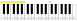
\includegraphics[width=1.0\linewidth]{figures/keyboard.png}
	\caption{Layout of the 37-key piano keyboard used in tests. Key names ($C1$, $C\#1$, $D1$ and so on) are overlayed on keys and yellow shapes on top of the keyboard represents the task/sound and $C3$-key labels.}
	\label{keyboard}
\end{figure}

\begin{figure}[h]
	\centering
	\includegraphics[width=1.0\linewidth]{figures/setup.png}
	\caption{Setup used in user tests. HapSynth is connected to the laptop with one \gls{usb} cable that relays both the \gls{midi} and serial data. Piano keyboard is connected to the laptop with a \gls{usb} cable. Audio interface is connected to the laptop with a \gls{usb} cable and to HapSynth and piano with audio cables.}
	\label{setup}
\end{figure}

Each participant had twelve tasks to complete. Tasks were grouped into four parts (indicated with letters $A$--$D$), where in each part a different force feedback mode was applied to the slider. Used force feedback modes were \textit{Detents}, \textit{Texture}, \textit{Friction}, and to draw comparison to \glspl{dmi} without force feedback, \textit{Position}. To counter learnability, different modes were applied to different parts for each participant, thus each participant experienced the modes in different order. \textit{Elasticity} and \textit{Oscillation} modes were left out from these tasks, as they don't allow leaving the slider to a set value, thus being unsuitable for the tasks.

Each task asked participants to change one or two given synthesis parameter values by moving the slider until the sound generated by HapSynth audibly matched to a pre-recorded sample. Each sample was recorded by setting HapSynth's parameters to the target value of a task programmatically and playing $C3$-key. Participants could listen to the pre-recorded sound by playing a key of the keyboard that was labelled with the task's number, and HapSynth by playing $C3$-key (or any un-labelled key, though $C3$-key is the one used for comparisons since that matches the pitch of the samples). Each part had three tasks with the following assignments always in the same order (so tasks 1, 4, 7, and 10 each had assignment 1, tasks 2, 5, 8, and 11 assignment 2 and so on):

\begin{enumerate}
	\item Change filter's cutoff frequency to match recorded sound
	\item Change envelope generator's attack time to match recorded sound
	\item Change LFO's frequency and oscillator's LFO amount to pulse width modulation to match recorded sound
\end{enumerate}

Table \ref{targets} shows the target value for each task. Value of 0 represents the slider in its left most position while 100 represents the right most position. With detents mode values 25 and 75 were one of the detents for each parameter (very easy to get exactly the right value), while 40 and 60 were not (impossible to get the right value). Values for tasks were designed so that no matter the order of the force feedback modes, in detents mode each participant would be able to get two values exactly right and two values would be impossible to get right. This allowed me to observe both the advantage and disadvantage that detent mode inherently causes and see whether those affected the participants' satisfaction and frustration, respectively.

\begin{table}[h!]
	\centering
	\begin{tabular}{|c||c|c||c|c|c|c|}
		\hline
		\multirow{3}{*}{\thead{Task}} & \multirow{3}{*}{\thead{Part}} & \multirow{3}{*}{\thead{\begin{tabular}[c]{@{}c@{}}Assign- \\ ment\end{tabular}}} & \multicolumn{4}{c|}{\thead{Target value (0-100)}} \\\cline{4-7}
			&&& \thead{Filter cutoff} & \thead{EG attack} & \thead{LFO fre-} & \thead{Oscillator LFO} \\
			&&& \thead{frequency} & \thead{time} & \thead{quency} & \thead{amount to PWM} \\
		\hline
		\hline
			1 & \multirow{3}{*}{$A$} & 1 & 60 & x & x & x \\ \cline{1-1} \cline{3-7}
			2 &                      & 2 & x & 25 & x & x \\ \cline{1-1} \cline{3-7}
			3 &                      & 3 & x & x & 40 & 75 \\
		\hline
		\hline
			4 & \multirow{3}{*}{$B$} & 1 & 40 & x & x & x \\ \cline{1-1} \cline{3-7}
			5 &                      & 2 & x & 60 & x & x \\ \cline{1-1} \cline{3-7}
			6 &                      & 3 & x & x & 75 & 25 \\
		\hline
		\hline
			7 & \multirow{3}{*}{$C$} & 1 & 25 & x & x & x \\ \cline{1-1} \cline{3-7}
			8 &                      & 2 & x & 75 & x & x \\ \cline{1-1} \cline{3-7}
			9 &                      & 3 & x & x & 60 & 40 \\
		\hline
		\hline
			10 & \multirow{3}{*}{$D$} & 1 & 75 & x & x & x \\ \cline{1-1} \cline{3-7}
			11 &                      & 2 & x & 40 & x & x \\ \cline{1-1} \cline{3-7}
			12 &                      & 3 & x & x & 25 & 60 \\
		\hline
	\end{tabular}
	\caption{Parts, assignments, and target synthesis parameter values for different tasks.}
	\label{targets}
\end{table}

When a participant thought they were as close to the target value as possible, they would announce that out loud. I measured the time the participant took in seconds and the distance(s) to the target value(s) in the units described above. These measurements were recorded for later analysis and not shown to the participant. If a participant took long time in one task, I asked them to stop and move to the next task. Results of these halted tasks were not included in the data analysis.

After each part I asked participants to fill out a \gls{nasa-tlx} load questionnaire to measure their perceived workload of the used force feedback mode. \gls{nasa-tlx} is developed by NASA in 1986 to evaluate workload using six dimensions: \textit{mental demand}, \textit{physical demand}, \textit{temporal demand}, \textit{own performance}, \textit{effort}, and \textit{frustration} (\cite{hart1986}). First, participants weight the relative importance of each dimension using pair-wise comparisons between them, and then they rate each dimension in a scale from 0 to 100 (higher number corresponding to higher workload). Finally, a weighted average is taken from the ratings giving the total score. (\cite{hart1986}). To shorten the duration of the user studies, I opted to utilize Raw TLX variation of \gls{nasa-tlx} which omits the weighting procedure of the dimensions (\cite{hart2006}). Omitting weighting has been shown both increasing and decreasing the sensitivity of the measurements, thus both methods seem equally valid (\cite{hart2006}).

Finally, after all the tests, I conducted a short interview. The interviews were semi-structured with open questions exploring the topics of overall experience using HapSynth, pros and cons of each individual mode, and benefits/drawbacks of having force feedback in a \gls{dmi} in general. Semi-structured interviews allow to focus into the topics that interest the participants and skip those that do not (\cite{lazar2017}), and with them I could gather more data with the limited sample size, thus I chose them for this study.

Along with the interviews I allowed the participants to freely use HapSynth to remind themselves how each of the force feedback modes felt. I also encouraged them to try out \textit{Elasticity} and \textit{Oscillation} modes, as they weren't part of the user tasks, but I was still interested to learn what the participants thought of them.

\section{Analysis methods}

User studies were analysed with qualitative and qualitative analysis methods. Interviews were analysed with thematic analysis using emergent coding, while one-way \glspl{anova} and pairwise comparisons were conducted for the \gls{nasa-tlx} and measured data from the tasks.

\textit{Qualitative data.} Thematic analysis using emergent coding was chosen for the analysis method of the interview data. Previous literature is relatively sparse on specifically \glspl{dmi} with force feedback, hence emergent coding was more appropriate method than priori coding (\cite{lazar2017}).

During the interviews participants' key observations were noted down, and later from the notes of all interviews repeating phenomena were identified and grouped into codes, such us "Force feedback assures user that the device is working" and "Too strong feedback can be unpleasant". These codes were grouped into concepts (i.e. "Force feedback helps user" and "Force feedback is unpleasant and hinders performance"), which were further grouped into categories ("Varying opinions on enjoyability and usefulness").

\textit{Quantitative data.} \gls{nasa-tlx} and measured data were analysed with statistical methods. For both one-way \gls{anova} tests were conducted with force feedback modes as independent variables. If some statistical significance was found from those, pairwise comparisons were used to further investigate the difference between the modes.

\chapter{Results and analysis}
\label{ch:results}
\section{Enjoyability and usefulness according to the interviews}

At the end of each user study a semi-structured interview was conducted with the participant. These interviews revealed widely diverging views towards the enjoyability and usefulness of force feedback with \glspl{dmi}. Some feedback modes polarized participants' opinions while others kept them relatively unanimous. Furthermore, participants came up with new force feedback modes for HapSynth, general improvements for the device, and potential target audiences.

\textit{Varying opinions on enjoyability and usefulness.} Participants provided diverse takes on enjoyability and usefulness of having force feedback on \glspl{dmi}. Several participants thought feeling the force feedback was simply fun, and many deemed force feedback useful, saying how it helped to assure the device is responding to user actions, gave one more sense to work with, and could be used to help guide the user towards a desired, possibly predefined, position, for example in a live situation. Accessibility benefits for people with disabilities or lack of perfect pitch was also brought up.

More reserved participants were worried about the limited usability of force feedback. They thought that the usable range between "not strong enough force feedback to have any benefit" to "too strong feedback it becomes irritating/hindering" would be quite small, and especially on stage situations the force feedback could easily be lost under the rumble of the shaky and noisy environment. Some participants were unable to tell whether force feedback brought more benefits or drawbacks.

In the negative end several participants thought force feedback either wasn't useful or actually lowered the enjoyability and usefulness of a \gls{dmi}. Participants said that the force feedback felt useless, especially in the current implementation where the opposing force is always constant, and for already musically skilled users. Furthermore, force feedback was described unpleasant and hindering, participants telling how it was not fun to use the device when it was fighting back, hurting the fingers, and how it felt like it didn't let the user move the slider to a position they wanted to move it to, thus obstructing the usage.

\textit{Position mode divided opinions.} \textit{Position} mode, which was used to compare force feedback modes to \glspl{dmi} without those, was seen both better and worse compared to the modes with force feedback. Some participants thought \textit{Position} mode was more pleasant to use after using modes with force feedback, and more useful as it didn't restrict movement at all. In contrary, some participants disliked \textit{Position} mode as it didn't provide any resistance and thus felt too "slippery".

\textit{Detents mode divided opinions.} Like \textit{Position}, \textit{Detents} mode also split the participants. Some thought it was fun to use, felt natural, and helped with the tasks since there was a limited discrete number of positions to choose from. On the contrary, others saw \textit{Detents} limiting as it prevented using values between two detents and thus not allowing to fine tune the value. The strength of \textit{Detents} mode's force feedback was also reported to be too strong, as the pressure it applies to the fingers rendered usage to what was described as "awful" and even "painful".

\textit{Texture mode felt good, but usefulness was indecisive.} \textit{Texture} mode was widely regarded as the most enjoyable feeling mode. Participants liked its smooth and natural feel, giving just enough feedback to assure the device is working, especially compared to usage without any force feedback. However, participants weren't as unanimous on whether having \textit{Texture} feedback was useful or not. The little resistance it gave was deemed helpful to find positions more gradually, but also made it feel like it was constantly "slightly off".

\textit{Friction mode was mostly disliked.} Most participants thought \textit{Friction} mode felt unpleasant and was hindering the usability, although few reported contrariwise. Like with \textit{Detents} mode the feedback was described as too strong. That made usage irritating, and painful, and giving the impression the user is doing something wrong, perhaps moving the slider to the wrong direction, thus hindering the usability. On the other hand, few participants liked the strong feedback and how it enabled to make small adjustments.

\textit{Elasticity and Oscillation modes were fun.} Even though the actual tasks did not use \textit{Elasticity} or \textit{Oscillation} modes, I still let participants to test them if they wanted to for additional feedback. Neither of these modes allow user to move the slider and leave it to that position, which some participants wished would have been possible. However, both modes were considered fun to use and potentially usable options for performing.

\textit{New force feedback modes and usability improvements were devised.} Participants came up with ideas for new feedback modes, and some general usability improvements for a \gls{dmi} with force feedback. Force feedback could be used to effectively guide the user towards a predetermined position, either by applying stronger feedback the further away the user is from that position, or the reverse, stronger feedback the closer user gets to the position. The feedback could also match the sound, either by replicating the generated audio wave or mimicking the feel of an existing instrument. Some variations for \textit{Detents} mode were suggested, such as applying the feedback in a sawtooth wave pattern. Furthermore, combining two or more existing modes was brought up, either by applying them at the same time, or by applying them for different ranges of the slider. Some usability improvements were brought up, for example it was suggested that the part which transmits the force feedback could be bigger, letting the user feel the feedback with larger surface area of their hand.

\textit{Thoughts on user groups.} According to the participants, force feedback on a \gls{dmi} would either be niche feature or something that would garner a wide audience. On one hand, force feedback could be used for learning purposes, being useful for users who are new to \glspl{dmi}, but on the other hand it was described as an enthusiast feature, only suitable for people with some special requirements. It was left unclear whether these two groups would be mutually exclusive or separate coexisting groups.

In conclusion, with these interviews alone nothing decisive can be said about the enjoyability or usefulness of a force feedback enabled \gls{dmi}. However, the positive comments do support the idea, and encourage for further research of the topic. \textit{Texture} mode seemed to rise above other modes in terms of enjoyability (including \textit{Position}), while usefulness (and possible hinderance) of \textit{Detents} mode was recognized.

\section{Enjoyability and usefulness according to \gls{nasa-tlx} measures}

One-way \gls{anova} tests were performed for all \gls{nasa-tlx} dimensions combined and for each dimension separately, comparing the effect of the different force feedback modes to the perceived load. \gls{anova} from the combined dimensions did not show statistical significance, $F(1.8, 25.7) = 3.1, p > 0.05$. Likewise \textit{mental demand}, \textit{temporal demand}, \textit{own performance}, \textit{effort}, and \textit{frustration} dimensions did not show statistical significance. Results of those are presented in Table \ref{tlx-anova}.

\begin{table}[h!]
	\centering
	\begin{tabular}{ |c|c| }
		\hline
		\thead{Dimension} & \thead{\gls{anova}} \\
		\hline
		Mental demand & $F(2.8, 38.8) = 0.2, p > 0.05$ \\
		\hline
		Physical demand & $F(2.1, 29.1) = 3.9, p < 0.05$ \\
		\hline
		Temporal demand & $F(2.4, 32.9) = 1.8, p > 0.05$ \\
		\hline
		Own performance & $F(2.7, 38.5) = 0.3, p > 0.05$ \\
		\hline
		Effort & $F(2.0, 27.5) = 2.5, p > 0.05$ \\
		\hline
		Frustration & $F(1.5, 21.7) = 1.7, p > 0.05$ \\
		\hline
	\end{tabular}
	\caption{\gls{anova} results of \gls{nasa-tlx} individual dimensions. Only \textit{physical demand} shows statistical significance.}
	\label{tlx-anova}
\end{table}

On the other hand, \gls{anova} test from \textit{physical demand} did show some statistical significance, with $F(2.1, 29.1) = 3.9, p < 0.05$. Pairwise comparisons were done to compare the effect of the force feedback modes to \textit{physical demand}, but none of the comparisons showed statistical significance. However, Figure \ref{tlx-physical-chart} hints that \textit{Detents} and \textit{Friction} modes would be physically more demanding than \textit{Position} and \textit{Texture} modes.

\begin{figure}[h!]
	\centering
	\includegraphics[width=1.0\linewidth]{figures/tlx-anova.png}
	\caption{Estimated Marginal Means of the force feedback modes to \textit{physical demand}.}
	\label{tlx-physical-chart}
\end{figure}

It can be extrapolated from these results that inclusion of force feedback in a \gls{dmi} does not significantly make its usage more or less demanding, excluding \textit{physical demand}, which might increase with some force feedback modes. Overall, with all \gls{nasa-tlx} dimensions, \textit{Texture} mode seemed to be slightly less demanding than \textit{Detents} and \textit{Friction} modes. These results seem to be in accordance with the interview results, \textit{Texture} mode being most liked possibly due to its lower demand, while \textit{Friction} mode's increase in especially \textit{physical demand} affecting the user experience in a negative way.

\section{Measured benefit}

Like for \gls{nasa-tlx}, one-way \gls{anova} tests were conducted for the measured time and accuracy data from the tasks, comparing the effect of the force feedback modes to time and accuracy, respectively. Results from neither of them showed any statistical significance, time being $F(2.7, 38.4) = 0.9, p > 0.05$ and accuracy $F(2.1, 29.3) = 0.9, p > 0.05$.

Based on these results there is no measurable benefit to time or accuracy from having force feedback in a \gls{dmi} in the context of the tasks of this user study. Like interviews and \gls{nasa-tlx} results, \textit{Friction} mode seemed to be slightly, albeit statistically insignificantly better than the other modes (including \textit{Position}). \textit{Detents} mode seemed to be the worst performing mode in both measures.

\chapter{Conclusion}
\label{ch:conclusion}
\section{Results and discussion}

In this study I aimed to research what kind of effect including force feedback could have to a \gls{dmi}. My research questions were how do users find helpfulness and enjoyability of using a \gls{dmi} with force feedback compared to using one without it, and whether the inclusion of force feedback provides any measurable benefit. As can be seen from Chapter \ref{ch:results}, the results of the study were mostly inconclusive. I couldn't find any statistically significant objective measurable benefit on the context of the tasks used in the user study, but on the other hand neither hinderance. This allows me to put more weight on the subjective views, especially from the interviews. Since force feedback wasn't obstructing the usage of a \gls{dmi}, and some participants enjoyed it and found it useful, it is worthwhile to think that when well implemented it could improve the user experience for some users.

\textit{Texture} mode garnered the most positive comments from the interviews, and it also performed the best in \gls{nasa-tlx} and measured data. Participants appreciated its ability to affirm the device is working, and the applied resistance it provided. Going by these results it's somewhat safe to say a \textit{Texture} mode like feature would be a welcomed addition to a \gls{dmi}.

\textit{Detents} mode has the clear use case of reducing options, which should make both finding a value and remembering past values easier, two pros participants brought up in the interviews. However, measured data showed that in the context of the tasks it did not perform any faster or more accurate than other modes, probably the contrary of that. Also, it is likely physically more demanding to use than without force feedback, so if implemented in an actual product the strength of the force feedback should be tuned to a suitable level. The identified benefits should still make it a worthwhile consideration when designing \glspl{dmi}. If included, the user should be provided with an option to leave the slider between two detents, for example by turning off the mode.

\textit{Friction} mode was both disliked in the interviews and performed poorly in the statistical tests. Factoring in the seemingly increased \textit{physical demand}, it is apparent that too strong force feedback negatively affects the user experience. This could explain why Fjeld et al. did not include the mode in their later publications. As is the mode would not be an enjoyable or useful addition to have.

\textit{Elasticity} and \textit{Oscillation} modes were said to be fun options for performance. Due to their nature, they were not suitable for the tasks, and thus lack \gls{nasa-tlx} results and measured data to evaluate. Fun performance factors should make them ideal inclusions for a \gls{dmi}, but as participants said they should also have an option to leave the slider to a desired position without it going back to the initial one.

These force feedback modes give justification to consider motorized inputs when designing a \gls{dmi}, and having a motorized input for even one mode inevitably affords possibility to include any number of modes, as it becomes a matter of software. However, adding that motorized input comes with a cost: the circuitry of the device becomes more complex, the power requirement increases, and the added components and engineering unavoidably increases the price of the product, possibly significantly. Evaluating whether the benefits match the increase in cost is left outside of the scope of this study. If force feedback modes are added to a \gls{dmi}, the strength of those should be user configurable to account for different preferences and usage environments. Users could also be able to turn off the force feedback completely.

\section{Reliability of the study}

This study was conducted without affiliations to 3rd parties and did not receive external funding. User studies were conducted within the premises of Tampere University. During and after these studies several issues arose concerning the reliability of the overall study, as described next.

The software and hardware of HapSynth used in the tests had several issues. For many participants, most likely due to problems in hardware, the force feedback was applied only when moving the slider to one direction but not to the other. In such cases I asked the participants to imagine that the force feedback was applied similarly to both directions.

Some participants had trouble navigating HapSynth on tasks that required modifying two parameters, which shifted their attention out of feeling the force feedback. For the purposes of those tasks, it would have been beneficial to have at least one more motorized slider, so users could have just edited both parameters at the same time without needing to navigate the device.

The test setup had other issues as well. The pre-recorded sounds and the sound generated by HapSynth never matched perfectly, even if the slider was on the same exact position used when recording the samples. This could have been caused by the sampling or routing of the devices, or possibly some other parameter than what the participant was changing was slightly off from the recording. This caused some unwanted frustration with some participants. Furthermore, all edited parameters were continuous in nature, but to best see the usefulness of \textit{Detents} mode, a discrete parameter should have been used for some tasks.

Finally, the number of participants was relatively low, and did not sufficiently represent the target audience of the device. More participants would have made the statistical tests more accurate and could have revealed some significance between the force feedback modes or level out the results completely to rule out the seeming differences. More participants could also have allowed to divide them into two separate groups, novice and expert users, which could have had different results. Now only a few participants had prior experience with \glspl{dmi}, while most were students of Haptic Interaction course and thus inherently had some interest towards haptic and force feedback but not necessarily \glspl{dmi}. To get broader, more representative results, more participants should have been recruited, especially ones with more experience using \glspl{dmi}.

\section{Future work}

The objective of this research was to explore the helpfulness and enjoyability of force feedback in a \gls{dmi}. Still, many questions remain that were left outside the scope of the study, or which rose from the findings. HapSynth, the open source force feedback enabled \gls{dmi} that was developed during this thesis, provides a starting point for answering such questions.

This research utilized a motorized slider to provide force feedback, but force feedback could also be provided in numerous other ways. As mentioned in Chapter \ref{ch:methodology}, aside from slider I also explored the possibility of providing force feedback through motorized knobs or piano keys, all of which could be interesting future research topics, expanding on this thesis and works such as \textcite{kirkegaard2020} and \textcite{timmermans2020}. Different mediums could utilize the same force feedback modes presented in this work, but also provide some new ones possibly unique for those mediums. Especially the prototype of \textcite{timmermans2020} was primarily used to replicate existing piano actions, but utilizing novel force feedback modes could bring up interesting new playing methods.

Furthermore, adding a second or even more motorized sliders to the device would open avenues for new interactions and related research. Operating multiple sliders simultaneously could yield interesting results, either by using the same or different force feedback modes on each slider. Also having the sliders affect each other in some way, i.e. similarly to \textcite{kontogeorgakopoulos2019} or \textcite{bak2015}, could yield exciting results.

Finally, having two sliders perpendicularly and coupled together would provide one more degree of freedom, forming a force feedback enabled XY pad. Exploring \gls{dmi} applications for such contraption would be fascinating.

%%%%% Bibliography/references.

% Print the bibliography according to the
% information in ./tex/references.bib and
% the in-line citations used in the body of
% the thesis.
% \emergencystretch=2em
\newrefcontext[sorting=nyt]
\printbibliography[heading=bibintoc]

%%%%% Appendices.

% Use only if it clarifies the structure of
% the document. Remember to introduce each
% appendix and its content.

\begin{appendices}

\chapter{External links}
\label{ch:links}
\section{HapSynth GitHub repository} \label{ch:github}
\url{https://github.com/SirMorland/HapSynth}
\section{YouTube video demonstrating HapSynth functionality} \label{ch:youtube}
\url{https://youtu.be/hl_LQ_ap-Gw}

\newgeometry{a4paper,
             top=2.5cm,
             bottom=2.5cm,
             left=0cm,
             right=0cm}
    \begin{landscape}
        \chapter{Button layout handout}
        \thispagestyle{empty}
        \label{ch:button}
        \begin{figure}[h]
	\centering
	\includegraphics[width=1.0\linewidth]{figures/cheat-sheet.png}
\end{figure}
    \end{landscape}
\restoregeometry

\newgeometry{a4paper,
             top=2.5cm,
             bottom=2.5cm,
             left=0cm,
             right=0cm}
    \begin{landscape}
        \chapter{Schematics}
        \thispagestyle{empty}
        \label{ch:schematics}
        \begin{figure}[h]
	\centering
	\includegraphics[width=0.8\linewidth]{figures/schematics-1.png}
\end{figure}

\begin{figure}[h]
	\centering
	\includegraphics[width=0.8\linewidth]{figures/schematics-2.png}
\end{figure}
    \end{landscape}
\restoregeometry

\newgeometry{a4paper,
             top=2.5cm,
             bottom=2.5cm,
             left=0cm,
             right=0cm}
    \begin{landscape}
        \chapter{Bill of materials}
        \thispagestyle{empty}
        \label{ch:bom}
        \begin{tabularx}{\linewidth}{lllXXXll}
	\csvreader[
		tabular=|lllXXXll|,
		no head,
		table head = \hline,
		late after first line = \\\hline,
		table foot = \hline,
		respect underscore = true,
		separator = semicolon
	]{../data/bom.csv}{}{%
		\ifnum\thecsvrow=18 \hline \fi%
		\csvcoli &%
		\csvcolii &%
		\csvcoliii &%
		\csvcoliv &%
		\csvcolv &%
		\csvcolvi &%
		\csvcolvii &%
		\csvcolviii %
	}
	\label{bom}
\end{tabularx}
    \end{landscape}
\restoregeometry

\end{appendices}

\end{document}